% (find-LATEX "2020-2-C2-somas-2.tex")
% (defun c () (interactive) (find-LATEXsh "lualatex -record 2020-2-C2-somas-2.tex" :end))
% (defun C () (interactive) (find-LATEXSH "lualatex 2020-2-C2-somas-2.tex" "Success!!!"))
% (defun D () (interactive) (find-pdf-page      "~/LATEX/2020-2-C2-somas-2.pdf"))
% (defun d () (interactive) (find-pdftools-page "~/LATEX/2020-2-C2-somas-2.pdf"))
% (defun e () (interactive) (find-LATEX "2020-2-C2-somas-2.tex"))
% (defun o () (interactive) (find-LATEX "2020-1-C2-somas-2.tex"))
% (defun u () (interactive) (find-latex-upload-links "2020-2-C2-somas-2"))
% (defun v () (interactive) (find-2a '(e) '(d)))
% (defun d0  () (interactive) (find-ebuffer "2020-2-C2-somas-2.pdf"))
% (defun cv () (interactive) (C) (ee-kill-this-buffer) (v) (g))
%          (code-eec-LATEX "2020-2-C2-somas-2")
% (find-pdf-page   "~/LATEX/2020-2-C2-somas-2.pdf")
% (find-sh0 "cp -v  ~/LATEX/2020-2-C2-somas-2.pdf /tmp/")
% (find-sh0 "cp -v  ~/LATEX/2020-2-C2-somas-2.pdf /tmp/pen/")
%     (find-xournalpp "/tmp/2020-2-C2-somas-2.pdf")
%   file:///home/edrx/LATEX/2020-2-C2-somas-2.pdf
%               file:///tmp/2020-2-C2-somas-2.pdf
%           file:///tmp/pen/2020-2-C2-somas-2.pdf
% http://angg.twu.net/LATEX/2020-2-C2-somas-2.pdf
% (find-LATEX "2019.mk")
% (find-CN-aula-links "2020-2-C2-somas-2" "2" "c2m202somas2" "c2m202s2")
%
% Video:
% (find-ssr-links "c2m202somas2" "2020-2-C2-somas-2")
% (code-video     "c2m202somas2video" "$S/http/angg.twu.net/eev-videos/2020-2-C2-somas-2.mp4")
% (find-c2m202somas2video  "0:00")
% (find-c2m202somas2video  "4:00")
% (find-c2m202somas2video  "6:30" "exercicio 1")
% (find-c2m202somas2video  "8:16" "")
% (find-c2m202somas2video  "9:10" "o ponto não pertence")
% (find-c2m202somas2video  "9:52" "e projetar eles no eixo vertical")
% (find-c2m202somas2video "10:15" "dá dois intervalos mas")
% (find-c2m202somas2video "10:34" "as pessoas que querem resolver tudo por contas")
% (find-c2m202somas2video "11:08" "as pessoas que querem resolver tudo por contas 2")
% (find-c2m202somas2video "12:46" "exercicio 2")
% (find-c2m202somas2video "16:07" "exercicio 5")
% (find-c2m202somas2video "17:16" "exercicio 6")
% (find-c2m202somas2video "18:32" "exercicio 7")
% (find-c2m202somas2video "20:00" "exercicio 8")

% (find-ssr-links "c2m202somas2b" "2020-2-C2-somas-2b")
% (code-video "c2m202somas2bvideo" "$S/http/angg.twu.net/eev-videos/2020-2-C2-somas-2b.mp4")
% (find-c2m202somas2bvideo "0:00")
% (find-c2m202somas2bvideo "2:44" "quando vocês conseguirem visualizar o L(C)")
% (find-c2m202somas2bvideo "3:00" "quando vocês conseguirem visualizar o L(C)")
% (find-c2m202somas2bvideo "3:30" "retângulo mais alto e retângulo mais baixo")
% (find-c2m202somas2bvideo "6:05" "exercicio 10")

% (find-ssr-links "c2m202somas2c" "2020-2-C2-somas-2c")
% (code-video "c2m202somas2cvideo" "$S/http/angg.twu.net/eev-videos/2020-2-C2-somas-2c.mp4")
% (find-c2m202somas2cvideo "0:00")
% (find-c2m202somas2cvideo "0:22" "sobre um exercicio que eu acabei de acrescentar")
% (find-c2m202somas2cvideo "1:30" "e aí eu peço pra vocês representarem graficamente")
% (find-c2m202somas2cvideo "1:58" "eu vou desenhar bem rápido")
% (find-c2m202somas2cvideo "2:43" "e quando eu peço pra vocês representarem a diferença")
% (find-c2m202somas2cvideo "3:12" "só que num gráfico só")
% (find-c2m202somas2cvideo "4:32" "essa parte em laranja")
% (find-c2m202somas2cvideo "6:01" "13b")
% (find-c2m202somas2cvideo "6:21" "áreas de trapézios")
% (find-c2m202somas2cvideo "6:58" "um argumento parecido mas para deslizar")
% (find-c2m202somas2cvideo "7:35" "recorta e cola com desliza")
% (find-c2m202somas2cvideo "8:16" "e agora tem essa parte mais difícil")
% (find-c2m202somas2cvideo "8:33" "estimativa")
% (find-c2m202somas2cvideo "8:50" "área do Mickey")
% (find-c2m202somas2cvideo "9:50" "uma coisa parecida pra essa figura feita de retângulos")
% (find-c2m202somas2cvideo "10:20" "a gente vai descobrir o que é essa base dela")
% (find-c2m202somas2cvideo "10:35" "a altura desse primeiro retângulo daqui")
% (find-c2m202somas2cvideo "10:50" "a soma de todos esses retangulinhos")

% (find-ssr-links "c2m202somas2d" "2020-2-C2-somas-2d")

% «.defs»			(to "defs")
% «.title»			(to "title")
% «.porque-aprender-isto»	(to "porque-aprender-isto")
% «.um-milhao-de-pontos»	(to "um-milhao-de-pontos")
% «.imagens-de-conjuntos»	(to "imagens-de-conjuntos")
% «.exercicio-1»		(to "exercicio-1")
% «.imagens-de-intervalos»	(to "imagens-de-intervalos")
% «.exercicio-2»		(to "exercicio-2")
% «.exercicio-3»		(to "exercicio-3")
% «.exercicio-4»		(to "exercicio-4")
% «.exercicio-5»		(to "exercicio-5")
% «.exercicio-6»		(to "exercicio-6")
% «.exercicio-7-novo»		(to "exercicio-7-novo")
% «.exercicio-8-novo»		(to "exercicio-8-novo")
% «.exercicio-9-novo»		(to "exercicio-9-novo")
% «.L-e-M»			(to "L-e-M")
% «.inf»			(to "inf")
% «.exercicio-8»		(to "exercicio-8")
% «.exercicio-9»		(to "exercicio-9")
% «.sup»			(to "sup")
% «.exemplao»			(to "exemplao")
% «.exercicio-10»		(to "exercicio-10")
% «.intover-intunder»		(to "intover-intunder")
% «.exercicio-11»		(to "exercicio-11")
% «.exercicio-12»		(to "exercicio-12")
% «.exercicio-13»		(to "exercicio-13")
% «.pierluigi»			(to "pierluigi")
%
% «.exercicio-1»		(to "exercicio-1")
% «.exercicio-2»		(to "exercicio-2")
% «.exercicio-7-sup»		(to "exercicio-7-sup")
%
% «.djvuize»	(to "djvuize")

\documentclass[oneside,12pt]{article}
\usepackage[colorlinks,citecolor=DarkRed,urlcolor=DarkRed]{hyperref} % (find-es "tex" "hyperref")
\usepackage{amsmath}
\usepackage{amsfonts}
\usepackage{amssymb}
\usepackage{pict2e}
\usepackage[x11names,svgnames]{xcolor} % (find-es "tex" "xcolor")
\usepackage{colorweb}                  % (find-es "tex" "colorweb")
%\usepackage{tikz}
%
% (find-dn6 "preamble6.lua" "preamble0")
%\usepackage{proof}   % For derivation trees ("%:" lines)
%\input diagxy        % For 2D diagrams ("%D" lines)
%\xyoption{curve}     % For the ".curve=" feature in 2D diagrams
%
\usepackage{edrx15}               % (find-LATEX "edrx15.sty")
\input edrxaccents.tex            % (find-LATEX "edrxaccents.tex")
\input edrxchars.tex              % (find-LATEX "edrxchars.tex")
\input edrxheadfoot.tex           % (find-LATEX "edrxheadfoot.tex")
\input edrxgac2.tex               % (find-LATEX "edrxgac2.tex")
%
%\usepackage[backend=biber,
%   style=alphabetic]{biblatex}            % (find-es "tex" "biber")
%\addbibresource{catsem-slides.bib}        % (find-LATEX "catsem-slides.bib")
%
% (find-es "tex" "geometry")
\usepackage[a6paper, landscape,
            top=1.5cm, bottom=.25cm, left=1cm, right=1cm, includefoot
           ]{geometry}
%
\begin{document}

\catcode`\^^J=10
\directlua{dofile "dednat6load.lua"}  % (find-LATEX "dednat6load.lua")

%L dofile "edrxtikz.lua"  -- (find-LATEX "edrxtikz.lua")
%L dofile "edrxpict.lua"  -- (find-LATEX "edrxpict.lua")
\pu

% «defs»  (to ".defs")
% (find-LATEX "edrx15.sty" "colors-2019")
\long\def\ColorRed   #1{{\color{Red1}#1}}
\long\def\ColorViolet#1{{\color{MagentaVioletLight}#1}}
\long\def\ColorViolet#1{{\color{Violet!50!black}#1}}
\long\def\ColorGreen #1{{\color{SpringDarkHard}#1}}
\long\def\ColorGreen #1{{\color{SpringGreenDark}#1}}
\long\def\ColorGreen #1{{\color{SpringGreen4}#1}}
\long\def\ColorGray  #1{{\color{GrayLight}#1}}
\long\def\ColorGray  #1{{\color{black!30!white}#1}}
\long\def\ColorBrown #1{{\color{Brown}#1}}
\long\def\ColorBrown #1{{\color{brown}#1}}
\long\def\ColorOrange#1{{\color{orange}#1}}

\long\def\ColorShort #1{{\color{SpringGreen4}#1}}
\long\def\ColorLong  #1{{\color{Red1}#1}}

\def\frown{\ensuremath{{=}{(}}}
\def\True {\mathbf{V}}
\def\False{\mathbf{F}}
\def\gr   {\mathsf{gr}}
\def\dom  {\mathsf{dom}}
\def\im   {\mathsf{im}}
\def\D    {\displaystyle}

\def\drafturl{http://angg.twu.net/LATEX/2020-2-C2.pdf}
\def\drafturl{http://angg.twu.net/2020.2-C2.html}
\def\draftfooter{\tiny \href{\drafturl}{\jobname{}} \ColorBrown{\shorttoday{} \hours}}



%  _____ _ _   _                               
% |_   _(_) |_| | ___   _ __   __ _  __ _  ___ 
%   | | | | __| |/ _ \ | '_ \ / _` |/ _` |/ _ \
%   | | | | |_| |  __/ | |_) | (_| | (_| |  __/
%   |_| |_|\__|_|\___| | .__/ \__,_|\__, |\___|
%                      |_|          |___/      
%
% «title»  (to ".title")
% (c2m202somas2p 1 "title")
% (c2m202somas2    "title")

\thispagestyle{empty}

\begin{center}

\vspace*{1.2cm}

{\bf \Large Cálculo 2 - 2020.2}

\bsk

Aula 4: Integrais como somas de retângulos (2)

\bsk

Eduardo Ochs - RCN/PURO/UFF

\url{http://angg.twu.net/2020.2-C2.html}

\end{center}

\newpage



{\bf Aproximações por cima e por baixo}

Uma das figuras na p.2 das notas da Cristiane Hernández é esta:

% (find-books "__analysis/__analysis.el" "hernandez")
% (find-c2crishernandezpage (+ 10  2) "")
% (find-latexgimp-links "2020-1-C2/area-hernandez-1")

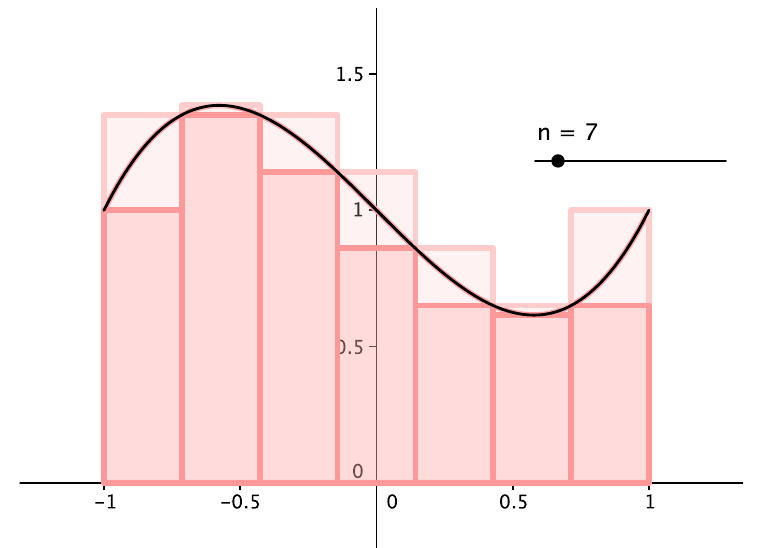
\includegraphics[width=6cm]{2020-1-C2/area-hernandez-1.png}

Ela mostra uma tentativa de calcular uma integral fazendo uma {\sl
  aproximação por retângulos por baixo} e uma {\sl aproximação por
  retângulos por cima} para $y=f(x)$ no intervalo entre $x=-1$ e
$x=1$. A curva $y=f(x)$ fica entre estas duas aproximações.

\newpage

% «porque-aprender-isto»  (to ".porque-aprender-isto")
% (c2m202somas2p 3 "porque-aprender-isto")
% (c2m202somas2    "porque-aprender-isto")

{\bf Porque aprender isto}

\ssk

As definições {\sl formais} de ``aproximação por retângulos por
baixo'' e ``aproximação por retângulos por cima'' são bem trabalhosas.
Elas envolvem alguns truques com conjuntos infinitos, ``para todo'' e
``existe'', que a maioria dos livros de Cálculo pula...

Nós vamos ver essas definições em detalhes porque entendê-las e
aprender a visualizar cada subexpressão delas vai acabar sendo
\ColorRed{muito} útil pras próximas matérias de Matemática do curso de
vocês.

No material da aula 2 eu pedi pra vocês aprenderem a fazer certos
desenhos sem contas, chamei isso de o ``jeito esperto'', e disse que
fazê-los calculando todas as coordenadas era o ``jeito burro''. Na
discussão desse material pelo Telegram a Eduarda me pediu pra explicar
melhor isso, e eu dei essa explicação aqui...

\newpage

% «um-milhao-de-pontos»  (to ".um-milhao-de-pontos")
% (c2m202somas2p 4 "um-milhao-de-pontos")
% (c2m202somas2    "um-milhao-de-pontos")

Tenta aprender a não fazer as contas... se você fizer tudo pelas
contas você vai demorar muito mais e não vai descobrir um monte de
truques importantes que a gente só descobre se a gente tenta aprender
a visualizar tudo geometricamente...

Acho que eu tenho um exemplo bom.

Num dos primeiros slides eu usei uma figura copiada das notas da
Cristiane Hernandez em que ela usa uma partição com 7 intervalos - ela
até escreveu do lado ``$n=7$''...

Daqui a pouco a gente vai ter que usar figuras --- que a gente não vai
poder desenhar explicitamente com todos os detalhes --- com 10
intervalos, ou 100, ou 1000, ou um milhão de intervalos

Se você aprender a visualizar tudo sem contas você vai conseguir
visualizar a figura com um milhão de intervalos em poucos segundos.

E se você tiver que fazer as contas pra um milhão de intervalos você
vai gastar um tempo que a gente não tem $\frown$



\newpage

% «imagens-de-conjuntos»  (to ".imagens-de-conjuntos")
% (c2m202somas2p 5 "imagens-de-conjuntos")
% (c2m202somas2    "imagens-de-conjuntos")

{\bf Imagens de conjuntos}

\ssk

Dê uma olhada na seção 1.3 do Martins/Martins.

% (find-martinscdipage (+ 10  18) "1.3 Grafico de uma funcao")

Nós vamos usar uma notação um pouco diferente da deles.

Se $f:A→\R$ (obs: $A=\dom(f)$),
%
$$\begin{array}{rcl}
  \gr_f    &=& \setofst{(x,f(x))}{x∈A}, \\
  \im_f    &=& \setofst{f(x)}{x∈A}, \\
  \gr_f(B) &=& \setofst{(x,f(x))}{x∈B}, \\
  F(B)     &=& \setofst{f(x)}{x∈B}, \\
  \end{array}
$$

\newpage

Por exemplo, se
%
$$\begin{array}{rrcl}
  f: & \R &\to& \R \\
     &  x &↦&   x^2 \\
  \end{array}
$$

e $B=\{-1,0,1,2\}$ então:
%
$$\begin{array}{rcl}
  \gr_f(B) &=& \gr_f(\{-1,0,1,2\}), \\
           &=& \setofst{(x,f(x))}{x∈\{-1,0,1,2\}} \\
           &=& \{(-1,f(-1)), (0,f(0)), (1,f(1)), (2,f(2))\} \\
           &=& \{(-1,(-1)^2), (0,0^2), (1,1^2), (2,2^2)\} \\
           &=& \{(-1,1), (0,0), (1,1), (2,4)\} \\[5pt]
  F(B)     &=& \setofst{f(x)}{x∈\{-1,0,1,2\}} \\
           &=& \{(-1)^2, 0^2, 1^2, 2^2\} \\
           &=& \{1, 0, 1, 4\} \\
           &=& \{0, 1, 4\} \\
  \end{array}
$$


\newpage

% «exercicio-1»  (to ".exercicio-1")
% (c2m202somas2p 7 "exercicio-1")
% (c2m202somas2    "exercicio-1")

Se visualizarmos $B$ como um subconjunto do eixo $x$

então $\gr_f(B)$ é o resultado de ``levantar'' cada ponto de $B$

para o ponto correspondente no gráfico de $f$,

e $F(B)$ é o resultado de projetar todos os pontos de $\gr_f(B)$

no eixo $y$.

\msk

{\bf Exercício 1.}

Sejam $f(x)=x^2$ e $B=\{\ColorRed{-3},\ColorRed{-2},-1,0,1,2\}$.

a) Calcule $F(B)$.

b) Calcule $\gr_f(B)$.

c) Represente graficamente num gráfico só: $B$ ``como um subconjunto
do eixo $x$'', $\gr_f(B)$, $F(B)$ ``como um subconjunto do eixo $y$''.

d) Represente graficamente num (outro) gráfico só: $B$ ``como um
subconjunto do eixo $\ColorRed{y}$'', $\gr_f(B)$, $F(B)$ ``como um
subconjunto do eixo $\ColorRed{y}$''.

% Pra representar o conjunto {-3,-2,-1,0,1,2} no eixo x você vai pôr bolinhas nestes pontos do R^2:
% {(-3,0),(-2,0),(-1,0),(0,0),(1,0),(2,0)}

% Pra representar o conjunto {-3,-2,-1,0,1,2} no eixo y você vai pôr bolinhas nestes pontos do R^2:
% {(0,-3),(0,-2),(0,-1),(0,0),(0,1),(0,2)}


\newpage

% «imagens-de-intervalos»  (to ".imagens-de-intervalos")
% (c2m202somas2p 8 "imagens-de-intervalos")
% (c2m202somas2    "imagens-de-intervalos")

{\bf Imagens de intervalos}

\ssk

% (find-LATEX "edrxpict.lua" "beginpicture")

Seja:

$f(x)=
    \unitlength=10pt
    \celllower=2.5pt%
    \def\cellfont{\scriptsize}%
    %
    \vcenter{\hbox{%
    \beginpicture(0,0)(11,7)
    \pictgrid%
    \pictpiecewise{(0,3)--(3,6)--(8,1)--(11,4)}%
    \put(3,6.5){\cell{(3,6)}}%
    \put(8,0.5){\cell{(8,1)}}%
    \pictaxes%
    \end{picture}%
    }}
    =
    \scalebox{1.0}{$
    \begin{cases}
    x+3 & \text{quando $x≤3$}, \\
    9-x & \text{quando $3<x<8$}, \\
    x-7 & \text{quando $8≤x$} \\
    \end{cases}
    $}
   $

\bsk


Se $B$ é um conjunto infinito ---

por exemplo, $B = [1,2) ∪ [6,7)$ ---

não dá pra calcularmos $\gr_f(B)$ e $F(B)$

fazendo as contas pra todos os pontos...

É melhor fazer desenhos.







\newpage

\phantom{a}

\vspace*{-1cm}

$%f(x)=
    \unitlength=25pt
    \celllower=2.5pt%
    \def\cellfont{\scriptsize}%
    %
    \vcenter{\hbox{%
    \beginpicture(0,0)(11,7)
    \pictgrid%
    \pictpiecewise{(0,3)--(3,6)--(8,1)--(11,4)}%
    \put(3,6.25){\cell{(3,6)}}%
    \put(8,0.75){\cell{(8,1)}}%
    \pictaxes%
    \ColorOrange{%
      %\linethickness{4pt}
      \pictpiecewise{(1,0)c--(2,0)o
                     (1,4)c--(2,5)o
                     (0,4)c--(0,5)o
                     (6,0)c--(7,0)o
                     (6,3)c--(7,2)o
                     (0,3)c--(0,2)o
                    }%
    }
    \end{picture}%
    }}
   $

\bsk

Neste caso temos

$F([1,2) ∪ [6,7)) = (2,3] ∪ [4,5)$.


\newpage

% «exercicio-2»  (to ".exercicio-2")
% (c2m202somas2p 10 "exercicio-2")
% (c2m202somas2     "exercicio-2")

{\bf Exercício 2.}

Seja $f$ a função definida dois slides atrás.

Calcule:

a) $F([2,3))$

b) $F([2,4))$

c) $F((2,4))$

d) $F((2,9))$

e) $F([1,2)∪[4,5))$

f) $F([1,2)∪\{3\}∪[4,5))$

\msk

\newpage

% «exercicio-3»  (to ".exercicio-3")
% (c2m202somas2p 11 "exercicio-3")
% (c2m202somas2     "exercicio-3")

{\bf Exercício 3.}

Para cada uma dos proposições abaixo diga

se ela é verdadeira ou falsa.

a) $∀x∈[7,9]. \, 1<f(x)$

b) $∀x∈[7,9]. \, 1≤f(x)$

c) $∃x∈[7,9]. \, 1<f(x)$

d) $∃x∈[7,9]. \, 1≤f(x)$

\newpage

% «exercicio-4»  (to ".exercicio-4")
% (c2m202somas2p 12 "exercicio-4")
% (c2m202somas2     "exercicio-4")


Da mesma forma que podemos definir funções

nós podemos definir proposições.

Uma proposição é uma função que retorna $\True$ ou $\False$.

Seja $P(y) = (∀x∈[7,9]. \, y≤f(x))$.

\msk

{\bf Exercício 4.}

Para cada uma das proposições abaixo

diga se ela é verdadeira ou falsa.

a) $P(0.5)$ 

b) $P(0.99)$ 

c) $P(1)$ 

d) $P(1.01)$ 

e) $P(2)$ 




\newpage

% «exercicio-5»  (to ".exercicio-5")
% (c2m202somas2p 13 "exercicio-5")
% (c2m202somas2     "exercicio-5")

{\bf Exercício 5.}

Calcule os dois conjuntos abaixo:

a) $L = \setofst{y∈\R}{∀x∈[7,9].\, y≤f(x)}$

b) $U = \setofst{y∈\R}{∀x∈[7,9].\, f(x)≤y}$

e:

c) Represente o conjunto $L$ no eixo $y$.

d) Represente o conjunto $U$ no eixo $y$.

e) Represente o conjunto $L$ usando notação de intervalos ---

algo como: ``$L = [42,99)∪\{200\}∪(420,+∞)$''.

f) Represente o conjunto $U$ usando notação de intervalos.

\newpage

% «exercicio-6»  (to ".exercicio-6")
% (c2m202somas2p 14 "exercicio-6")
% (c2m202somas2     "exercicio-6")

{\bf Exercício 6.}

Seja $M(y) = (y∈L \text{ e } ∀y'∈L.\,y'≤y)$ ---

ou, equivalentemente, $M(y) = (y∈L \text{ e } ∀z∈L.\,z≤y)$.

Para cada uma das proposições abaixo

diga se ela é verdadeira ou falsa.

a) $M(4)$

b) $M(2)$

c) $M(0)$

d) $M(0.5)$

e) $M(1)$



\newpage

% «exercicio-7-novo»  (to ".exercicio-7-novo")
% (c2m202somas2p 15 "exercicio-7-novo")
% (c2m202somas2     "exercicio-7-novo")

{\footnotesize \ColorRed{(Obs: este slide é uma versão melhorada do slide do exercício 7!)}}

Alguns slides atrás nós definimos:
%
$$\begin{array}{rcl}
  L    &=& \setofst{y∈\R}{∀x∈[7,9].\, y≤f(x)} \\
  M(y) &=& (y∈L \text{ e } ∀z∈L.\,z≤y) \\
  \end{array}
$$

Agora vamos generalizar o $L$ de dois jeitos:
%
$$\begin{array}{rcl}
     L(B) &=& \setofst{y∈\R\ColorRed{\,∪\,\{-∞,+∞\}}}{∀b∈B.\, y≤f(b)} \\
     I(C) &=& \setofst{y∈\R\ColorRed{\,∪\,\{-∞,+∞\}}}{∀c∈C.\, y≤c} \\
 % N(y,D) &=& (y∈D \text{ e } ∀z∈D.\,z≤y) \\
  \end{array}
$$

{\bf Exercício 7':}

a) Calcule $L([7,9])$.

b) Verifique que $L([7,9]) = I(F([7,9]))$.

c) $L(B) = I(F(B))$ vai ser verdade pra qualquer conjunto $B$? Porquê?

%   M(y,C) &=& (y∈L(C) \text{ e } ∀z∈L(C).\,z≤y) \\
%  L(F(B)) &=& \setofst{y∈\R\ColorRed{\,∪\,\{-∞,+∞\}}}{∀x∈B.\, y≤f(x)} \\


\newpage

% «exercicio-8-novo»  (to ".exercicio-8-novo")
% (c2m202somas2p 16 "exercicio-8-novo")
% (c2m202somas2     "exercicio-8-novo")

{\footnotesize \ColorRed{(Obs: este slide é uma versão melhorada do slide do exercício 8!)}}

Agora vamos generalizar o $M$ e definir o inf...
%
$$\begin{array}{rcl}
     L(B) &=& \setofst{y∈\R\ColorRed{\,∪\,\{-∞,+∞\}}}{∀b∈B.\, y≤f(b)} \\
     I(C) &=& \setofst{y∈\R\ColorRed{\,∪\,\{-∞,+∞\}}}{∀c∈C.\, y≤c} \\
   M(y,D) &=& (y∈D \text{ e } ∀d∈D.\,d≤y) \\
  \text{$y$ é o inf de $C$} &=& (y∈I(C) \text{ e } ∀d∈I(C).\,d≤y) \\
  \end{array}
$$



{\bf Exercício 8':}

a) Calcule $I([2,3])$ e $I((2,3))$.

b) Calcule $M(1,[-∞,2])$, $M(2,[-∞,2])$, $M(3,[-∞,2])$.

c) Calcule o valor de ``1 é o inf de \{2,3,4\}''. Deve dar $𝐛V$ ou $𝐛F$.

d) Calcule ``2 é o inf de \{2,3,4\}'' e ``3 é o inf de \{2,3,4\}''.

e) Calcule $I(\R)$.

f) Calcule $I(∅)$.





\newpage

% «exercicio-9-novo»  (to ".exercicio-9-novo")
% (c2m202somas2p 17 "exercicio-9-novo")
% (c2m202somas2     "exercicio-9-novo")

{\footnotesize \ColorRed{(Obs: este slide é uma versão melhorada do slide do exercício 9!)}}

Agora vamos definir o sup:
%
$$\begin{array}{rcl}
     U(B) &=& \setofst{y∈\R\ColorRed{\,∪\,\{-∞,+∞\}}}{∀b∈B.\, f(b)≤y} \\
     S(C) &=& \setofst{y∈\R\ColorRed{\,∪\,\{-∞,+∞\}}}{∀c∈C.\, c≤y} \\
   N(y,D) &=& (y∈D \text{ e } ∀d∈D.\,y≤d) \\
  \text{$y$ é o sup de $C$} &=& (y∈S(C) \text{ e } ∀d∈S(C).\,y≤d) \\
  \end{array}
$$

{\bf Exercício 9':}

a) Calcule $S([2,3])$ e $S((2,3))$.

b) Calcule $N(2,[3,+∞])$, $N(3,[3,+∞])$, $N(4,[3,+∞])$.

c) Calcule o valor de ``5 é o sup de \{2,3,4\}''. Deve dar $𝐛V$ ou $𝐛F$.

d) Calcule ``3 é o sup de \{2,3,4\}'' e ``4 é o sup de \{2,3,4\}''.

e) Calcule $S(\R)$.

f) Calcule $S(∅)$.







\newpage

% «L-e-M»  (to ".L-e-M")
% (c2m202somas2p 15 "L-e-M")
% (c2m202somas2     "L-e-M")

Alguns slides atrás nós definimos:
%
$$\begin{array}{rcl}
  L    &=& \setofst{y∈\R}{∀x∈[7,9].\, y≤f(x)} \\
  M(y) &=& (y∈L \text{ e } ∀z∈L.\,z≤y) \\
  \end{array}
$$

Agora vamos generalizar isto para:
%
$$\begin{array}{rcl}
  L(C) &=& \setofst{y∈\R\ColorRed{\,∪\,\{-∞,+∞\}}}{∀x∈C.\, y≤f(x)} \\
  M(y,C) &=& (y∈L(C) \text{ e } ∀z∈L(C).\,z≤y) \\
  \end{array}
$$

{\bf Exercício 7.}

Calcule:

a) $L((2,3]∪[4,5))$

b) $M(0,\, (2,3]∪[4,5))$

c) $M(1,\, (2,3]∪[4,5))$

d) $M(2,\, (2,3]∪[4,5))$

e) $M(3,\, (2,3]∪[4,5))$


% Bom, agora que a gente sabe que
% L((2,3]∪[4,5)) = [-∞,4]
% a gente pode reescrever o
% M(0, (2,3]∪[4,5))
% como :
% (0∈[-∞,4] e ∀z∈[-∞,4].z≤0)
% 
% E aí:
% 0∈[-∞,4] é verdadeiro
% ∀z∈[-∞,4].z≤0 é falso
% (0∈[-∞,4] e ∀z∈[-∞,4].z≤0) é falso

\newpage

% «inf»  (to ".inf")
% (c2m202somas2p 16 "inf")
% (c2m202somas2     "inf")

% «exercicio-8»  (to ".exercicio-8")
% (c2m202somas2p 16 "exercicio-8")
% (c2m202somas2     "exercicio-8")

E agora vamos definir o ``ínfimo'' de um conjunto $C$:
%
$$\begin{array}{rcl}
  L(C) &=& \setofst{y∈\R ∪ \{-∞,+∞\}}{∀x∈C.\, y≤f(x)} \\
                    M(y,C) &=& (y∈L(C) \text{ e } ∀z∈L(C).\,z≤y) \\
  y\text{ é o $\inf$ de C} &=& (y∈L(C) \text{ e } ∀z∈L(C).\,z≤y) \\
  \end{array}
$$

\msk

{\bf Exercício 8.}

Para cada uma das proposições abaixo 

diga se ela é verdadeira ou falsa.

a) 1 é o inf de $(2,3]∪[4,5)$

b) 2 é o inf de $(2,3]∪[4,5)$

c) 3 é o inf de $(2,3]∪[4,5)$

d) 0 é o inf de $\R$

e) $-∞$ é o inf de $\R$

f) $-∞$ é o inf de $∅$

g) $+∞$ é o inf de $∅$


\newpage

% «exercicio-9»  (to ".exercicio-9")
% (c2m202somas2p 17 "exercicio-9")
% (c2m202somas2     "exercicio-9")

{\bf Exercício 9.}

\ssk

Vamos definir $L(C)$ da seguinte forma:
%
$$L(C) = \setofst{y∈\R∪\{-∞,∞\}}{∀c∈C.\,y≤c}$$

Calcule:

a) $L([2,3])$

b) $L(\{2,3\})$

c) $L([2,3))$

d) $L((2,3))$ \;\; (repare que este (2,3) é um intervalo aberto!)

e) $L((-4,-3))$ \;\; (idem!)

f) $L(\R)$

g) $L(\R∪\{-∞,+∞\})$

h) $L(∅)$



\newpage

% «sup»  (to ".sup")
% (c2m202somas2p 18 "sup")
% (c2m202somas2     "sup")

E agora vamos definir o ``supremo'' de um conjunto $C$.

Compare:
%
$$\begin{array}{rcl}
  L(C) &=& \setofst{y∈\R ∪ \{-∞,+∞\}}{∀x∈C.\, y≤f(x)} \\
                    M(y,C) &=& (y∈L(C) \text{ e } ∀z∈L(C).\,z≤y) \\
  y\text{ é o $\inf$ de C} &=& (y∈L(C) \text{ e } ∀z∈L(C).\,z≤y) \\[5pt]
  %
  U(C) &=& \setofst{y∈\R ∪ \{-∞,+∞\}}{∀x∈C.\, f(x)≤y} \\
                   M'(y,C) &=& (y∈U(C) \text{ e } ∀w∈U(C).\,y≤w) \\
  y\text{ é o $\sup$ de C} &=& (y∈U(C) \text{ e } ∀w∈U(C).\,y≤w) \\
  \end{array}
$$

Infs e sups vão nos permitir definir o ``retângulo mais alto sob a
curva $y=f(x)$'' e o ``retângulo mais baixo sobre a curva $y=f(x)$''
de um modo que funciona até quando a $f$ é descontínua...

Veja o ``exemplão'' da próxima página.

\newpage

% «exemplao»  (to ".exemplao")
% (c2m202somas2p 19 "exemplao")
% (c2m202somas2     "exemplao")

{\bf Exemplão: métodos do sup e do inf}

\long\def\ColorUpper #1{{\color{red!20!white}#1}}
\long\def\ColorUpperB#1{{\color{red!30!white}#1}}
\long\def\ColorLower #1{{\color{red!40!white}#1}}
\long\def\ColorLowerB#1{{\color{red!50!white}#1}}

\msk

%\phantom{a}

%\vspace*{-1cm}

Seja
$f(x)=
    \unitlength=10pt
    \celllower=2.5pt%
    \def\cellfont{\scriptsize}%
    %
    \vcenter{\hbox{%
    \beginpicture(0,0)(5,6)
    \pictgrid%
    \ColorUpper {\polygon*(1,5)(3,5)(3,0)(1,0)}%
    \ColorUpperB{\polygon (1,5)(3,5)(3,0)(1,0)}%
    \ColorLower {\polygon*(1,1)(3,1)(3,0)(1,0)}%
    \ColorLowerB{\polygon (1,1)(3,1)(3,0)(1,0)}%
    \pictpiecewise{(0,3)--(2,5)o (2,3)c (2,1)o--(5,4)}%
    %\put(3,6.25){\cell{(3,6)}}%
    %\put(8,0.75){\cell{(8,1)}}%
    \pictaxes%
    \ColorRed{%
      %\linethickness{4pt}
      \pictpiecewise{(1,0)c--(3,0)c
                     (1,4)c--(2,5)o (2,3)c (2,1)o--(3,2)c
                     (0,4)c--(0,5)o (0,3)c (0,1)o--(0,2)c
                    }%
    }
    \end{picture}%
    }}
    =
    \scalebox{1.0}{$
    \begin{cases}
    x+3 & \text{quando $x<2$}, \\
    3   & \text{quando $x=2$}, \\
    x-1 & \text{quando $2<x$}. \\
    \end{cases}
    $}
   $

\msk

$\begin{array}{lrcl}
 \text{Seja}  &        B   &=& [1,3]. \\
 \text{Então} &      F(B)  &=& (1,2)∪\{3\}∪[4,5), \\
              &    U(F(B)) &=& [5,+∞], \\
              &    L(F(B)) &=& [-∞,1], \\
              & \sup(F(B)) &=& 5, \\
              & \inf(F(B)) &=& 1, \\
 \end{array}
$

\msk

$\sup(F([1,3]))·(3-1) $ é o retângulo mais claro, 

$\inf(F([1,3]))·(3-1) $ é o retângulo mais escuro... 



\newpage

% «exercicio-10»  (to ".exercicio-10")
% (c2m202somas2p 20 "exercicio-10")
% (c2m202somas2     "exercicio-10")

{\bf Exercício 10.}

\ssk

Seja:

$f(x)=
    \unitlength=10pt
    \celllower=2.5pt%
    \def\cellfont{\scriptsize}%
    %
    \vcenter{\hbox{%
    \beginpicture(0,0)(11,7)
    \pictgrid%
    \pictpiecewise{(0,3)--(3,6)--(8,1)--(11,4)}%
    \put(3,6.5){\cell{(3,6)}}%
    \put(8,0.5){\cell{(8,1)}}%
    \pictaxes%
    \end{picture}%
    }}
    =
    \scalebox{1.0}{$
    \begin{cases}
    x+3 & \text{quando $x≤3$}, \\
    9-x & \text{quando $3<x<8$}, \\
    x-7 & \text{quando $8≤x$} \\
    \end{cases}
    $}
   $

\msk

Seja $P = \{1,2,4,5,7,9,10\}$.

Represente graficamente:

\ssk

a) $\sum_{i=1}^{N} \inf(F([a_i,b_i]))·(b_i-a_i)$

b) $\sum_{i=1}^{N} \sup(F([a_i,b_i]))·(b_i-a_i)$

Dica: represente o (a) e o (b) no mesmo gráfico usando retângulos de
cores diferentes, como nas figuras das páginas 2 e 19.

\newpage

% «intover-intunder»  (to ".intover-intunder")
% (c2m202somas2p 21 "intover-intunder")
% (c2m202somas2     "intover-intunder")

{\bf Aproximações por cima e por baixo}

\ssk

Na aula 1 nós vimos esta figura:

$$\Intx{a}{b}{f(x)} = \Area \left(
  \myvcenter{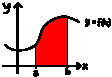
\includegraphics[width=2cm]{2020-1-C2/area-intro-1.pdf}}
  \right)
$$

As aproximações da integral de $f$ por retângulos por cima e por baixo
dependem da escolha de uma partição $P$ do intervalo $[a,b]$. As
definições formais são:
%
\def\Intover #1#2{\overline {∫}_{#1}#2\,dx}
\def\Intunder#1#2{\underline{∫}_{#1}#2\,dx}
\def\Intoverunder#1#2{\Intover{#1}{#2} - \Intunder{#1}{#2}}
%
\def\Intxover #1#2#3{\overline {∫}_{x=#1}^{x=#2}#3\,dx}
\def\Intxunder#1#2#3{\underline{∫}_{x=#1}^{x=#2}#3\,dx}
%
$$\begin{array}{rcl}
  \D \Intover {P}{f(x)} &=& \sum_{i=1}^{N} \sup(F([a_i,b_i]))·(b_i-a_i) \\[12pt]
  \D \Intunder{P}{f(x)} &=& \sum_{i=1}^{N} \inf(F([a_i,b_i]))·(b_i-a_i) \\
  \end{array}
$$



\newpage

% «exercicio-11»  (to ".exercicio-11")

{\bf Exercício 11.}

\ssk

Seja $f(x)$ a função do exercício 10.

Seja $P = \{1, 2, 3, \ldots, 10\}$.

Represente graficamente (num gráfico só)
%
$$f(x), \quad \D \Intunder {P}{f(x)}, \quad \D \Intover {P}{f(x)}.$$

A diferença entre as duas aproximações, $\D \Intover {P}{f(x)} - \D \Intunder {P}{f(x)}$,

corresponde à área em rosa claro nos slides 2 e 19.

Ela consiste num certo número de quadrados $1×1$.

\ColorRed{Quantos?}

\newpage

% «exercicio-12»  (to ".exercicio-12")
% (c2m202somas2p 23 "exercicio-12")
% (c2m202somas2     "exercicio-12")

{\bf Exercício 12.}

\ssk

Faça a mesma coisa, mas agora para a partição

$P = \{1, 1.5, 2, 2.5, \ldots, 10\}$.

\ssk

Agora a diferença $\D \Intover {P}{f(x)} - \D \Intunder {P}{f(x)}$

\ssk

é feita de um certo número de quadrados

de dimensões $0.5×0.5$.

\ColorRed{Quantos?}


\newpage

% «exercicio-13»  (to ".exercicio-13")
% (c2m202somas2p 24 "exercicio-13")
% (c2m202somas2     "exercicio-13")

{\bf Exercício 13.}

\ssk

Sejam:

$f(x) = 4 - (x-2)^2$,

$P_0 = \{0,4\}$,

$P_1 = \{0,2,4\}$,

$P_2 = \{0,1,2,3,4\}$,

$P_3 = \{0,0.5,1,1.5, \ldots, 4\}$.

a) Represente graficamente $\D \Intover {P_3}{f(x)} - \D \Intunder {P_3}{f(x)}$.

\newpage

{\bf Exercício 13 (cont.)}

\ssk

b) Represente \ColorRed{num gráfico só}:

$\Intx{0}{4}{f(x)}$,

$\Intoverunder {P_0}{f(x)}$,

$\Intoverunder {P_1}{f(x)}$,

$\Intoverunder {P_2}{f(x)}$,

$\Intoverunder {P_3}{f(x)}$.

\msk

c) Seja $A = \Intoverunder {P_3}{f(x)}$, considerado como um
subconjunto de $\R^2$ formado de retângulos, e $B$ o conjunto obtido a
partir de $A$ deslizando cada retângulo de $A$ pra baixo como
explicado no vídeo. Desenhe $B$ direito e obtenha uma estimativa para
a área de $B$ seguindo as idéias do vídeo.

\newpage

{\bf Exercício 13 (cont.)}

\ssk

d) Faça a mesma coisa que no item c, mas usando a partição $P_4$.

Você deve obter algo desta forma:
%
$$0 \le \Area(
  % (find-latexscan-links "C2" "20210225_retangulinhos")
  \myvcenter{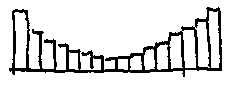
\includegraphics[height=0.5cm]{2020-2-C2/20210225_retangulinhos.pdf}}
  ) \le \_\_,
$$

onde o ``$\_\_$'' é ou um número ou uma expressão fácil de calcular.

\msk

e) Faça a mesma coisa que no item d, mas usando a partição $P_5$.

f) Faça a mesma coisa que no item d, mas usando a partição $P_6$.




\newpage

{\bf Exercício 14.}

\ssk

Repare que dá pra expressar a partição que divide o intervalo

$[a,b]$ em $N$ partes iguais assim:
%
$$\{a, \; a+1·\frac{b-a}{N},
       \; a+2·\frac{b-a}{N}, \ldots,
       \; a+N·\frac{b-a}{N}\}
$$

a) Teste a fórmula acima para o caso $[a,b]=[2,5]$, $N=6$.

b) Teste a fórmula acima para o caso $[a,b]=[2,5]$, $N=7$.

\msk

Dica importante: no Ensino Médio os professores dizem pra sempre fazer
``simplificações'' como esta aqui: $2 + 4·\frac{5-2}{7} =
\frac{26}{7}$. Em casos como a acima essas ``simplificações'' fazem
com que os padrões fiquem muito mais difíceis de entender.
\ColorRed{Não seja como aqueles professores do Ensino Médio!}

\newpage

{\bf Exercício 14 (cont.)}

\ssk

Se estamos tentando integrar uma função no intervalo $[a,b]$

a nossa \ColorRed{sequência preferida de partições} para este
intervalo

vai ser definida por:
%
$$P_k = \{ a, \; a + 1·\frac{b-a}{2^k}, \; a + 2·\frac{b-a}{2^k}, \ldots, b \}$$


c) A partição $P_0$ tem quantos intervalos? E quantos pontos?

d) A partição $P_1$ tem quantos intervalos? E quantos pontos?

e) A partição $P_2$ tem quantos intervalos? E quantos pontos?

f) A partição $P_5$ tem quantos intervalos? E quantos pontos?



\newpage

{\bf Mais definições}

\ssk

Defs:
%
$$\begin{array}{rcl}
  \D \Intxover {a}{b}{f(x)} &=& \D \lim_{k→∞} \Intover{P_k}{f(x)} \text{ e} \\[16pt]
  \D \Intxunder{a}{b}{f(x)} &=& \D \lim_{k→∞} \Intunder{P_k}{f(x)}, \\
  \end{array}
$$

onde $P_0, P_1, P_2, P_3, \ldots$ é a nossa sequência preferida de
partições

para o intervalo $[a,b]$, que definimos no slide anterior.

\newpage

{\bf Exercício 15.}

\ssk

Seja $f(x) = 4 - (x-2)^2$.

a) Represente graficamente $\Intxover {0}{4}{f(x)}$, representando

todas as ``$\Intover{P_k}{f(x)}$''s num gráfico só.

b) Represente graficamente $\Intxunder {0}{4}{f(x)}$, representando

todas as ``$\Intunder{P_k}{f(x)}$''s num gráfico só.




\newpage

% «pierluigi»  (to ".pierluigi")
% (c2m202somas2p 34 "pierluigi")
% (c2m202somas2     "pierluigi")
% (find-books "__analysis/__analysis.el" "beneveri")

{\bf As notas do Pierluigi Benevieri}

\ssk

Agora dê uma olhada nestas notas

de Cálculo 2 do Pierluigi Benevieri:

\ssk

\url{https://www.ime.usp.br/~pluigi/registro-MAT121-15.pdf}

\ssk

Nas páginas 3 e 4 ele define a integral (na definição 3) usando a
``família de todas as partições do intervalo $[a,b]$''... isto é
beeeem mais difícil de entender e visualizar do que o que eu fiz aqui,
usando o limite na minha sequência preferida de partições do intervalo
$[a,b]$...

\newpage

{\bf Exercício 16.}

\ssk

a) Entenda a definição da Função de Dirichlet que o Pierluigi faz nas
páginas 8 e 9, e que ele chama de $f(x)$ naquele trecho das notas.

b) Faça o gráfico dessa função $f(x)$.

\msk

Seja $[a,b]=[2,5]$.

c) Represente graficamente $\Intover{P_k}{f(x)}$ e
$\Intunder{P_k}{f(x)}$

para $k=0$, $k=1$ e $k=2$.

d) Convença-se de que 
%
$$\Intxover {2}{5}{f(x)} = 3 \quad \text{e} \quad
  \Intxunder{2}{5}{f(x)} = 0.
$$

% https://www.ime.usp.br/~pluigi/registro-MAT121-15.pdf
% (code-pdf-page "pierluigi" "$S/https/www.ime.usp.br/~pluigi/registro-MAT121-15.pdf")
% (code-pdf-text "pierluigi" "$S/https/www.ime.usp.br/~pluigi/registro-MAT121-15.pdf")
% (find-pierluigipage)
% (find-pierluigipage 3)
% (find-pierluigipage 8)
% (find-pierluigitext)





\newpage

{\bf A definição de integral}

\ssk

\def\eqa{\overset{\ColorRed{\Downarrow}}{=}}

A nossa definição de $\Intx{a}{b}{f(x)}$ vai ser:
%
$$\Intx     {a}{b}{f(x)} \;\;=\;\;
  \Intxover {a}{b}{f(x)} \;\; \eqa \;\;
  \Intxunder{a}{b}{f(x)}
$$

se a igualdade marcada com `$\eqa$' for verdade.

\msk
\msk

Se a igualdade `$\eqa$' for falsa vamos dizer que:

``$f(x)$ não é integrável no intervalo $[a,b]$'',

``$\Intx{a}{b}{f(x)}$ não está definida'', ou

``$\Intx{a}{b}{f(x)}$ dá erro''.

\msk
\msk

(Compare com $\frac{42}{0}$...)


\newpage

{\bf Outra função não integrável}

\ssk

A função de Dirichlet não é integrável porque

ela é ``muito descontínua''.

Um outro exemplo de função não integrável é:
%
$$g(x) = \begin{cases}
    x^{-2} & \text{quando $x≠0$}, \\
    0      & \text{quando $x=0$}. \\
    \end{cases}
$$

{\bf Exercício 17.}

a) Calcule $g(2)$, $g(1)$, $g(\frac12)$, $g(\frac1{10})$,

$g(-2)$, $g(-1)$, $g(-\frac12)$, $g(-\frac1{10})$, $g(0)$.

b) Calcule $\lim_{x→0^+} g(x)$ e $\lim_{x→0^-} g(x)$.

c) Calcule $\lim_{x→_+∞} g(x)$ e $\lim_{x→-∞} g(x)$.

d) Faça o gráfico da $g(x)$.



\newpage

{\bf Exercício 17 (cont.)}

Seja $[a,b] = [-2,2]$.

\msk

e) Represente graficamente $\Intover{P_k}{g(x)}$ e
$\Intunder{P_k}{g(x)}$

para $k=0$, $k=1$ e $k=2$.

\msk

f) Convença-se de que $\Intover{P_k}{g(x)} = +∞$ para todo $k$

e de que $\Intunder{P_k}{g(x)} ≥ 0$ para todo $k$.

\bsk

Quando nós aprendermos o Teorema Fundamental do Cálculo

(p.12 das notas do Pierluigi!) nós vamos ver que se aplicarmos

ele a esta $g(x)$ obtemos um resultado que não faz sentido:
%
$$\Intx{-1}{1}{g(x)} = -2$$


\newpage



(Tudo a partir desta página é do material de 2020.1 e vai ser
totalmente reescrito!)

\newpage




{\bf Exercício 1.}

Leia a definição de integral definida do Martins/Martins e tente
entendê-la. Dica: ela é ambígua e muito incompleta! A definição deles,
na p.203, é esta:
%
$$\int_a^b f(x)dx = \lim_{Δx_i→0} \sum_{i=1}^{n} f(x)Δx_i$$

por exemplo, o Martins/Martins dá uma definição bem incompleta de
integral na p.203 dele, e diz ``para detalhes consulte o livro do
Leithold''...

% (find-martinscdipage (+ 10 203) "6.5        Integral Definida")
% (find-martinscditext (+ 10 203) "6.5        Integral Definida")



\newpage

% (find-books "__analysis/__analysis.el" "martins-martins")

Martins/Martins: ``Elementos de cálculo diferencial e integral''

\url{http://angg.twu.net/2020.2-C2/martins_martins__cap_1.pdf}








\newpage

% «exercicio-1»  (to ".exercicio-1")
% (c2m202somas2p 3 "exercicio-1")
% (c2m202somas2    "exercicio-1")

{\bf Exercício 1.}

Sejam $g(x)=5-x$ e $P=\{1,2,4\}$.

Considere a expressão abaixo:
%
$$\sum_{i=1}^N g(b_i)(b_i-a_i)
  ≤ \Intx{1}{4}{g(x)}
  ≤ \sum_{i=1}^N g(a_i)(b_i-a_i)
  \qquad
  (*)
$$

a) Represente graficamente o primeiro somatório e calcule-o.

b) Represente graficamente o segundo somatório e calcule-o.

c) Represente graficamente a integral $\Intx{1}{4}{g(x)}$ como a área
sob a curva $y=g(x)$ entre $x=1$ e $x=4$ e calcule-a -- lembre que
vimos no final da aula passada como calcular áreas de trapézios.

d) Verifique que os dois `$≤$'s em $(*)$ são verdade.

e) Represente os dois somatórios e a integral num gráfico só.


\newpage

{\bf Exercício 1 (continuação).}

\ssk

f) O primeiro somatório está todo abaixo da curva $y=g(x)$? A curva
$y=g(x)$ está toda abaixo do segundo somatório? Se ``sim'' e ``sim''
represente os dois somatórios e a integral num gráfico só fazendo uma
figura parecida com a do slide 2, inclusive usando cores diferentes
para a área sob a aproximação por baixo (o somatório da esquerda) e a
aproximação por cima (o somatório da direita).


\newpage

Nos próximos exercícios nós vamos encontrar modos de fazer
aproximações por retângulos ``por cima'' e ``por baixo''. As nossas
primeiras tentativas vão ser meio bugadas e vai ser preciso
consertá-las.

Lembre que na aula passada nós vimos como visualizar vários somatórios
diferentes, e os que apareceram no exercício 1 correspondem à ``soma à
direita'' e a ``soma à esquerda'' desta página da Wikipedia:

\ssk

\url{https://pt.wikipedia.org/wiki/Soma_de_Riemann}

\newpage

% (c2m192p 3 "retangulos")
% (c2m192    "retangulos")

{\bf Algumas abreviações}

\def\sumiN#1{\sum_{i=1}^N #1 (b_i-a_i)}
\def\mname#1{\text{[#1]}}

$$\begin{array}{ccl}
  \mname{L}    &=& \sumiN {f(a_i)} \\
  \mname{R}    &=& \sumiN {f(b_i)} \\
  \mname{Trap} &=& \sumiN {\frac{f(a_i) + f(b_i)}{2}} \\
  \mname{M}    &=& \sumiN {f(\frac{a_i+b_i}{2})} \\
  \mname{min}  &=& \sumiN {\min(f(a_i), f(b_i))} \\
  \mname{max}  &=& \sumiN {\max(f(a_i), f(b_i))} \\
  % [5pt]
  % \mname{inf}  &=& \sumiN {\inf (\setofst{f(x)}{x∈[a_i,b_i]}) } \\
  % \mname{sup}  &=& \sumiN {\sup (\setofst{f(x)}{x∈[a_i,b_i]}) } \\
  % [5pt]
  % \overline \int_P f(x) \, dx &=& \sumiN {\sup (\setofst{f(x)}{x∈[a_i,b_i]}) } \\
  % \underline\int_P f(x) \, dx &=& \sumiN {\inf (\setofst{f(x)}{x∈[a_i,b_i]}) } \\
\end{array}
$$

Obs: todos os ``métodos'' acima, $\mname{L}$, $\mname{R}$,
$\mname{Trap}$, $\mname{M}$, $\mname{min}$, e $\mname{max}$, aparecem
na página da Wikipedia, mas com outros nomes e usando partições em que
todos os subintervalos têm o mesmo comprimento!

\newpage

% «exercicio-2»  (to ".exercicio-2")
% (c2m202somas2p 7 "exercicio-2")
% (c2m202somas2    "exercicio-2")

{\bf Exercício 2.} Seja $f$ a nossa função preferida (a da aula
passada!) e $P$ a partição $P=\{1,1.5,2,3,4\}$.

a) Represente em um gráfico só a função $f$ e $\mname{M}$.

b) Represente em um gráfico só a função $f$ e $\mname{min}$.

c) Represente em um gráfico só a função $f$ e $\mname{max}$.

\bsk

{\bf Exercício 3.} Faça um gráfico como o do item (f) do exercício 1
para
%
$$\mname{min} ≤ \Intx{1}{4}{f(x)} ≤ \mname{max}.$$

\bsk

{\bf Exercício 4.} Faça um gráfico como o do exercício anterior, mas
agora usando $P=\{1,1.5,3,4\}$. \ColorRed{Desta vez um trecho do
  gráfico de $y=f(x)$ vai ficar acima do \mname{max}!!!}



\newpage

{\bf A imagem de um conjunto por uma função}

Sejam:
%
$$\begin{array}{rcl}
  A &=& \{1,1.5,2,3\} \\
  B &=& \setofst{(x,f(x))}{x∈A} \\ 
    &=& \{ (1,f(1)), (1.5,f(1.5)), (2,f(2)), (3,f(3)) \} \\ 
  C &=& \setofst{f(x)}{x∈A} \\ 
    &=& \{ f(1), f(1.5), f(2), f(3) \} \\ 
  \end{array}
$$

Dá pra desenhar todos esses conjuntos num gráfico só bem rápido.

Instruções: desenhe o gráfico de $y=f(x)$; represente $A$ no eixo $x$;
desenhe $B$ em $\R^2$ ``levantando os pontos de $A$ para a curva de
$y=f(x)$''; represente $C$ \ColorRed{no eixo $y$} ``projetando os
pontos de $B$ no eixo $y$''.

\msk

{\bf Exercício 5.} Faça esse gráfico.

{\bf Exercício 6.} Faça a mesma coisa, mas com $A=[1,3.5]$, que é um
conjunto \ColorRed{infinito}... agora o conjunto $C$ vai ser um
intervalo. Qual?

\newpage

{\bf Um abuso de linguagem}

\ssk

A nossa função $f$ preferida é
%
$$\begin{array}{rrcl}
  f: & \R &→& \R \\
     &  x &↦& 4-(x-2)^2 \\
  \end{array}
$$

O domínio dela é $\R$, e isso quer dizer que se ela receber qualquer
argumento que não é um elemento de $\R$ ela deve dar erro...

Existe um truque tradicional que nos permite escrever a imagem de um
conjunto por uma função de um jeito mais curto. Se $A⊆\R$ é um
conjunto,
%
$$ f(A) = \setofst{f(a)}{a∈A} $$

É como se estivéssemos definindo uma função $f$ nova a partir da $f$
original, e as duas tem o mesmo nome mas domínios disjuntos -- a
original só lida com argumentos que são números reais, e a nova só
lida com argumentos que são conjuntos de números.


\newpage

% «exercicio-7-sup»  (to ".exercicio-7-sup")
% (c2m202somas2p 10 "exercicio-7-sup")
% (c2m202somas2     "exercicio-7-sup")

{\bf Sup}

\ssk

A função $\sup$ é uma espécie de generalização do $\mathsf{max}$.

Vamos começar com um exemplo. No exercício 6 você ``calculou'' -- por
desenhos e olhômetro -- $f([1,3.5])$, e você obteve um intervalo no
eixo $y$. Sejam $A=[1,3.5]$ e $C=f(A)$. Seja
%
$$D = \setofst{y∈\R∪\{-∞,+∞\}}{∀c∈C.\, c≤y}.$$

{\bf Exercício 7.} É verdade que $4∈D$?

{\bf Exercício 8.} É verdade que $5∈D$?

{\bf Exercício 9.} É verdade que $2∈D$?

{\bf Exercício 10.} É verdade que $+∞∈D$?

{\bf Exercício 11.} É verdade que $-∞∈D$?

{\bf Exercício 12.} Represente graficamente o conjunto $D$.

{\bf Exercício 13.} Qual é o menor elemento de $D$?

\newpage

{\bf Sup (2)}

\ssk

A definição \ColorRed{formal} do $\sup$ é \ColorRed{bem} complicada...

Dê uma olhada nesta página da Wikipedia, como curiosidade:

\ssk

\url{https://pt.wikipedia.org/wiki/Supremo_e_\%C3\%ADnfimo}

\ssk

Quando $C⊆\R$ temos um procedimento pra calcular $\sup(C)$ que é
equivalente à definição ``oficial'' complicadíssima que aparece na
Wikipedia. Ele funciona assim: defina
%
$$D = \setofst{y∈\R∪\{-∞,+∞\}}{∀c∈C.\, c≤y}.$$

Este conjunto $D$ vai ter duas propriedades importantes:

1) se $d∈D$ então $[d,+∞)⊆D$, e

2) $D$ tem um menor elemento.

\msk

O resultado de $\sup(C)$ vai ser o menor elemento de $D$.

\newpage

{\bf Sup e Inf}

\ssk

A definição \ColorRed{informal} abaixo também funciona:

Se $C⊆\R$ então $\sup(C)$ é o menor elemento de $\R∪\{-∞,∞\}$ que está
``\ColorRed{acima}'' de todos os elementos de $C$.

\msk

e, similarmente...

\msk

Se $C⊆\R$ então $\inf(C)$ é o maior elemento de $\R∪\{-∞,∞\}$ que está
``\ColorRed{abaixo}'' de todos os elementos de $C$.


\bsk


{\bf Exercício 14.} Calcule:

\def\foo#1{$\sup(#1)$ e $\inf(#1)$}

a) \foo{\{2,3,4\}}

b) \foo{[2,4]}

c) \foo{(2,4)}

d) \foo{\R}

e) \foo{∅}

\newpage


{\bf Algumas abreviações (2)}

\def\sumiN#1{\sum_{i=1}^N #1 (b_i-a_i)}
\def\mname#1{\text{[#1]}}

$$\begin{array}{ccl}
  \mname{L}    &=& \sumiN {f(a_i)} \\
  \mname{R}    &=& \sumiN {f(b_i)} \\
  \mname{Trap} &=& \sumiN {\frac{f(a_i) + f(b_i)}{2}} \\
  \mname{M}    &=& \sumiN {f(\frac{a_i+b_i}{2})} \\
  \mname{min}  &=& \sumiN {\min(f(a_i), f(b_i))} \\
  \mname{max}  &=& \sumiN {\max(f(a_i), f(b_i))} \\
  [5pt]
  \mname{inf}  &=& \sumiN {\inf (f([a_i,b_i]) } \\
  \mname{sup}  &=& \sumiN {\sup (f([a_i,b_i]) } \\
  % [5pt]
  % \overline \int_P f(x) \, dx &=& \sumiN {\sup (\setofst{f(x)}{x∈[a_i,b_i]}) } \\
  % \underline\int_P f(x) \, dx &=& \sumiN {\inf (\setofst{f(x)}{x∈[a_i,b_i]}) } \\
\end{array}
$$

Os métodos $\mname{inf}$ e  $\mname{sup}$ são novos...

Eles correspondem ao que a página da Wikipedia chama de ``Soma de
Riemann Inferior'' e ``Soma de Riemann Superior''.



\newpage

{\bf Uma versão ``consertada'' do exercício 4}

\ssk

{\bf Exercício 15.} Seja $P=\{1,1.5,3,4\}$. Faça um gráfico como o do
item (f) do exercício 1 para
%
$$\mname{inf} ≤ \Intx{1}{4}{f(x)} ≤ \mname{sup}.$$

e verifique que agora a curva $y=f(x)$ está entre $\mname{inf}$ e
$\mname{sup}$.







%\printbibliography

\GenericWarning{Success:}{Success!!!}  % Used by `M-x cv'

\end{document}

%  ____  _             _         
% |  _ \(_)_   ___   _(_)_______ 
% | | | | \ \ / / | | | |_  / _ \
% | |_| | |\ V /| |_| | |/ /  __/
% |____// | \_/  \__,_|_/___\___|
%     |__/                       
%
% «djvuize»  (to ".djvuize")
% (find-LATEXgrep "grep --color -nH --null -e djvuize 2020-1*.tex")

 (eepitch-shell)
 (eepitch-kill)
 (eepitch-shell)
# (find-fline "~/2020.2-C2/")
# (find-fline "~/LATEX/2020-2-C2/")
# (find-fline "~/bin/djvuize")

cd /tmp/
for i in *.jpg; do echo f $(basename $i .jpg); done

f () { rm -fv $1.png $1.pdf; djvuize $1.pdf }
f () { rm -fv $1.png $1.pdf; djvuize WHITEBOARDOPTS="-m 1.0" $1.pdf; xpdf $1.pdf }
f () { rm -fv $1.png $1.pdf; djvuize WHITEBOARDOPTS="-m 0.5" $1.pdf; xpdf $1.pdf }
f () { rm -fv $1.png $1.pdf; djvuize WHITEBOARDOPTS="-m 0.25" $1.pdf; xpdf $1.pdf }
f () { cp -fv $1.png $1.pdf       ~/2020.2-C2/
       cp -fv        $1.pdf ~/LATEX/2020-2-C2/
       cat <<%%%
% (find-latexscan-links "C2" "$1")
%%%
}

f 20210225_retangulinhos



%  __  __       _        
% |  \/  | __ _| | _____ 
% | |\/| |/ _` | |/ / _ \
% | |  | | (_| |   <  __/
% |_|  |_|\__,_|_|\_\___|
%                        
% <make>

 (eepitch-shell)
 (eepitch-kill)
 (eepitch-shell)
# (find-LATEXfile "2019planar-has-1.mk")
make -f 2019.mk STEM=2020-2-C2-somas-2 veryclean
make -f 2019.mk STEM=2020-2-C2-somas-2 pdf

% Local Variables:
% coding: utf-8-unix
% ee-tla: "c2m202somas2"
% End:
